\documentclass{article}
\usepackage{tikz}

\begin{document}
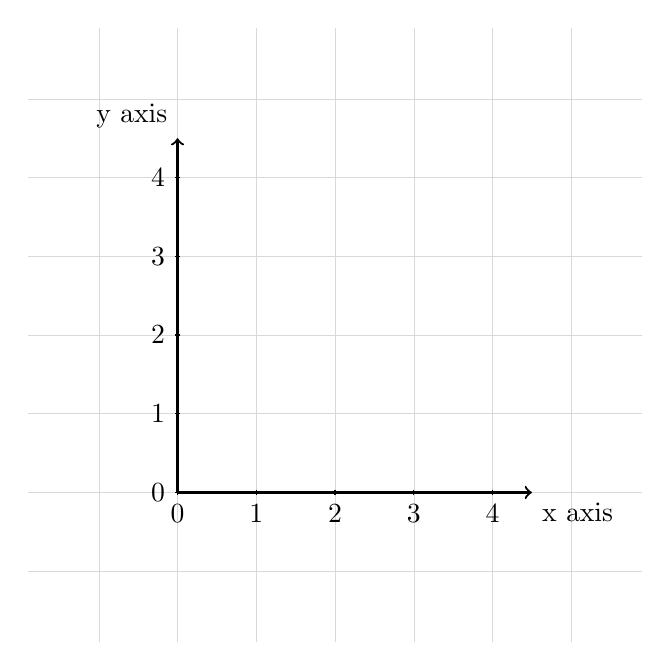
\begin{tikzpicture}
	\draw[step=1cm,gray!30,very thin] (-1.9,-1.9) grid (5.9,5.9);
	\draw[thick,->] (0,0) -- (4.5,0) node[anchor=north west]{x axis};
	\draw[thick,->] (0,0) -- (0,4.5) node[anchor=south east]{y axis};
	\foreach \x in {0,1,2,3,4}
	\draw(\x cm,1pt) -- (\x cm,-1pt) node[anchor=north] {$\x$};
	\foreach \y in {0,1,2,3,4}
	\draw(1pt,\y cm) -- (-1pt,\y cm) node[anchor=east] {$\y$};
\end{tikzpicture}
\end{document}
